% This file was created with tikzplotlib v0.10.1.
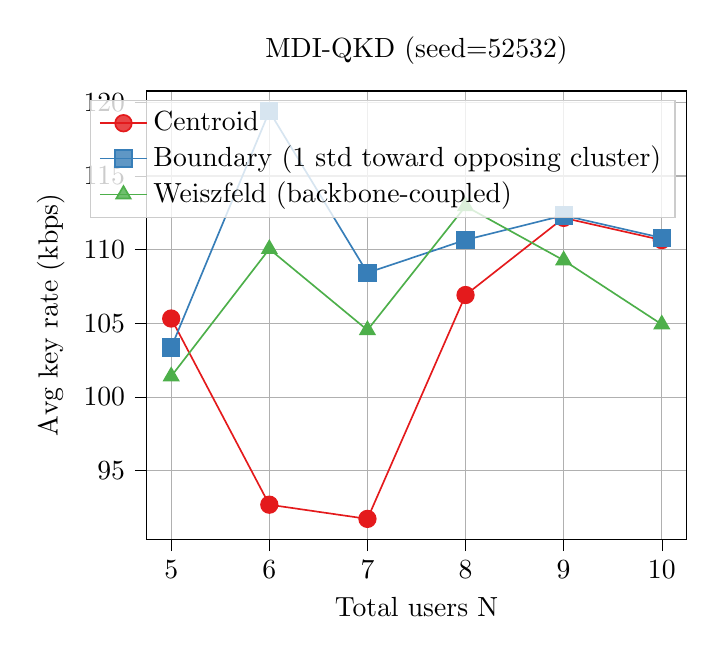
\begin{tikzpicture}

\definecolor{crimson2282628}{RGB}{228,26,28}
\definecolor{darkgray176}{RGB}{176,176,176}
\definecolor{lightgray204}{RGB}{204,204,204}
\definecolor{mediumseagreen7717574}{RGB}{77,175,74}
\definecolor{steelblue55126184}{RGB}{55,126,184}

\begin{axis}[
legend cell align={left},
legend style={fill opacity=0.8, draw opacity=1, text opacity=1, draw=lightgray204},
tick align=outside,
tick pos=left,
title={MDI-QKD (seed=52532)},
x grid style={darkgray176},
xlabel={Total users N},
xmajorgrids,
xmin=4.75, xmax=10.25,
xtick style={color=black},
xtick={4,5,6,7,8,9,10,11},
xticklabels={
  \(\displaystyle {4}\),
  \(\displaystyle {5}\),
  \(\displaystyle {6}\),
  \(\displaystyle {7}\),
  \(\displaystyle {8}\),
  \(\displaystyle {9}\),
  \(\displaystyle {10}\),
  \(\displaystyle {11}\)
},
y grid style={darkgray176},
ylabel={Avg key rate (kbps)},
ymajorgrids,
ymin=90.3504903576525, ymax=120.771895508575,
ytick style={color=black},
ytick={90,95,100,105,110,115,120,125},
yticklabels={
  \(\displaystyle {90}\),
  \(\displaystyle {95}\),
  \(\displaystyle {100}\),
  \(\displaystyle {105}\),
  \(\displaystyle {110}\),
  \(\displaystyle {115}\),
  \(\displaystyle {120}\),
  \(\displaystyle {125}\)
}
]
\addplot [semithick, crimson2282628, mark=*, mark size=3, mark options={solid}]
table {%
5 105.329619572735
6 92.6969171092329
7 91.7332815008762
8 106.92377648472
9 112.158329338999
10 110.652452953029
};
\addlegendentry{Centroid}
\addplot [semithick, steelblue55126184, mark=square*, mark size=3, mark options={solid}]
table {%
5 103.363575248183
6 119.389104365351
7 108.429877838862
8 110.664978504296
9 112.325360026757
10 110.804799308587
};
\addlegendentry{Boundary (1 std toward opposing cluster)}
\addplot [semithick, mediumseagreen7717574, mark=triangle*, mark size=3, mark options={solid}]
table {%
5 101.4069801808
6 110.046578271879
7 104.544305002582
8 112.948719033818
9 109.279193228686
10 104.930130596979
};
\addlegendentry{Weiszfeld (backbone-coupled)}
\end{axis}

\end{tikzpicture}
